(j). (4 points) \textsl{Recall the definition of hubs and authorities. Compute the hub and authority score of each actor, and for each phase. (Remember to load the adjacency data again this time using create\_using = nx.DiGraph().)}\\
\textsl{With networkx you can use the nx.algorithms.link\_analysis.hits function, set max\_iter=1000000 for best results.}\\
\textsl{Using this, what relevant observations can you make on how the relationship between n1 and n3 evolves over the phases. Can you make comparisons to your results in Part (g)?  ($\sim$300 words, 400 word limit.)}\\

\textbf{Solution}:\\
Hubs and authorities are defined for directed networks. Hubs point to authorities. Nodes have a high hub centrality if they point to many important authorities. Inversely, nodes have a high authority centrality if they have many nodes from where they are pointed to.\cite{networks_an_introduction}\\

For this problem the graphs for each phase had been recalculated with directed networks. The next step is the calculation of the corresponding hub and authority centralities for each node. Here a numpy array was initialized with zeros, such that the centrality is zero if the actual node is not mentioned in the current phase (or network).\\

The diagram in figure \ref{fig:hubs_authorities} shows the hub and authority centrality of node no. 1 and node no. 3 over the phases 1 to 11. Overall, the node no. 1 has a higher centrality than node no. 3. Over long periods the hub centrality (outgoing messages) is high, and for two phases (6 and 7) the authority centrality (incoming messages) is high. In each phase the centrality is greater compared to node no. 3.\\

\begin{figure}[h]
	\centering
	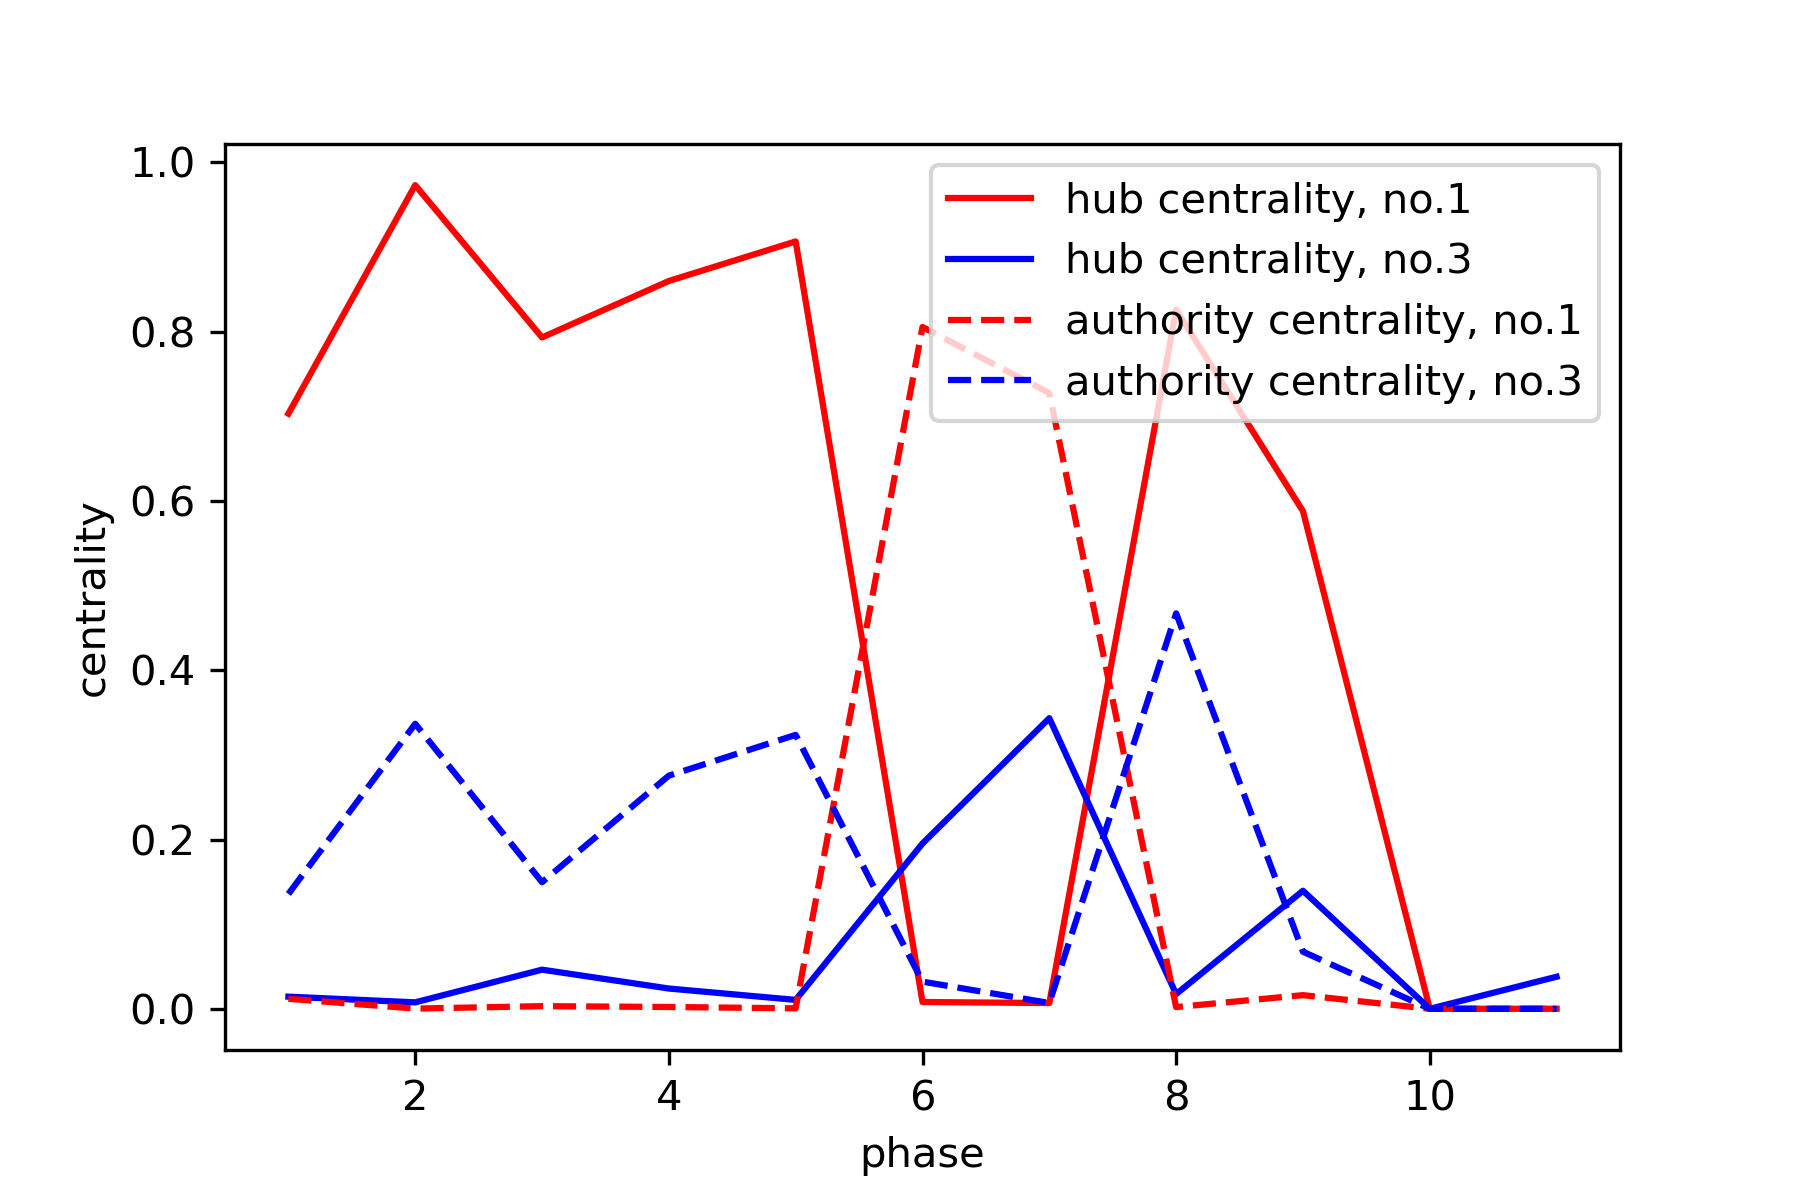
\includegraphics[width=0.7\linewidth]{problem_02/hubs_authorities}
	\caption{Hub and authority centrality for nodes no.1 and no.2}
	\label{fig:hubs_authorities}
\end{figure}

For both nodes there is the correlation that the hub centrality increases with an decreasing authority centrality, vice versa (see figure \ref{fig:hubs_authorities}). Moreover, the centralities for both nodes seem to be correlated as well. When there is an decrease in hub centrality for node no. 1 the hub centrality of node no. 3 increases. The same pattern can be found for the authority centrality. In other words, if for example the importance of outgoing messages of node no. 1 is reduced (in phases of high value seizures) the importance of outgoing massages of node no. 3 increases. Node no. 3 seem to overtake some of the importance of node no. 1 in these phases. In context of the introduction this makes perfect sense, due to the position of node no. 3 in the CAVIAR network. He is the principal lieutenant of node no. 1 and in close contact to this position. He might even work as a substitute for node no. 1 in phases of costly seizures.\\
